\section{이론적 배경}


\subsection{연구에 사용한 망원경}

본 연구에서 사용되는 망원경은 기존 천체관측에 있어서 큰 어려움은 없어 원격 천체관측을 진행할 수 있어야 하며, 직접 덮개를 개발하게 되므로 적절한 크기를 가지고 있어야 한다. 최종적으로 선발된 망원경은 Takahashi 사의 'FSQ-106ED'이다. Takahashi 사의 웹사이트에서 참고한 FSQ-106ED의 스펙은 Fig. \ref{FSQ}를 참고할 때 망원경의 경통은 580mm/675mm의 길이를 가지고 있으며, 지름은 125mm으로 마스크를 위한 덮개를 제작할 적절한 크기를 가지고 있다.

\begin{figure}[h]
	\begin{center}
		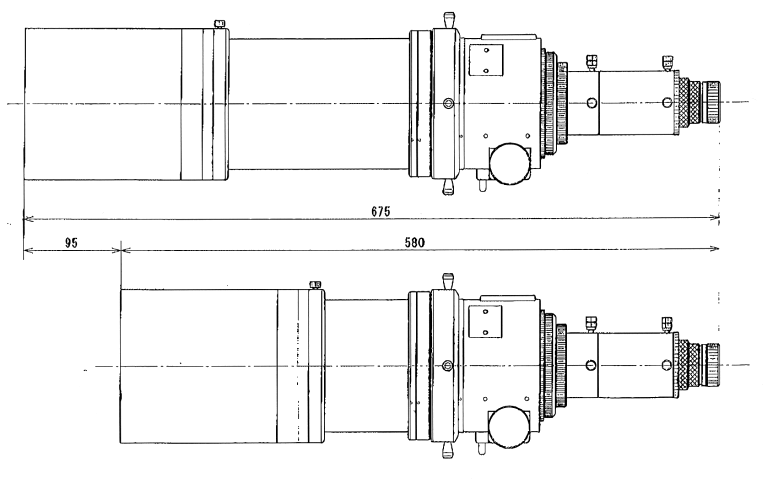
\includegraphics[width = 9cm]{FSQ_106ED_tube}
	\end{center}
	\caption{Takahashi 사의 웹사이트(https://www.takahashi-europe.com/en/FSQ-106ED.specifications.php)에서 참조한 FSQ-106ED의 스펙}
	\label{FSQ}
\end{figure}

\subsection{바흐티노프 마스크}

바흐티노프 마스크(Bahtinov mask)는 러시아의 아마추어 천문학자인 바흐티노프가 고안한 마스크 중 하나로, 기존에 사용하던 하트만 마스크(Hartmann mask)의 여러 단점을 보완하였기 때문에 이후 주류가 된 마스크의 종류이다. 두 마스크 모두 빛의 회절 현상을 이용한다는 공통점이 있지만, 천체관측에서는 바흐티노프 마스크가 더 포괄적으로 사용된다. 

빛의 회절은 직진하던 빛이 좁은 틈, 슬릿이나 장애물을 통과할 때 물체의 뒤편까지 빛이 나가는 현상으로, 슬릿의 폭이 좁을수록 회절이 잘 일어난다. 바흐티노프 마스크는 Fig. \ref{bahtinov}와 같이 방향이 어긋나있는 세 줄의 회절 슬릿들이 일렬로 나있는 모양을 가지고 있으며, 평행 광선인 별에서 오는 빛이 이러한 모양의 슬릿을 통과하면 빛은 좁은 틈에서 회절하게 된다. 빛은 좁은 방향으로 많이 회절하기 때문에 슬릿을 통과한 빛은 통과한 슬릿에 수평한 방향의 선 모양 상을 만들게 된다. 초점이 올바르지 않은 경우에는 평행광이 한점에 모이지 않기 때문에 세 개의 선이 한 점에서 만나지 않지만, 초점이 정확하게 맞추어진 경우에는 상들이 한 점에서 모이기 때문에 세 개의 선이 한 점에서 만나게 된다.

\begin{figure}[h]
	\begin{center}
		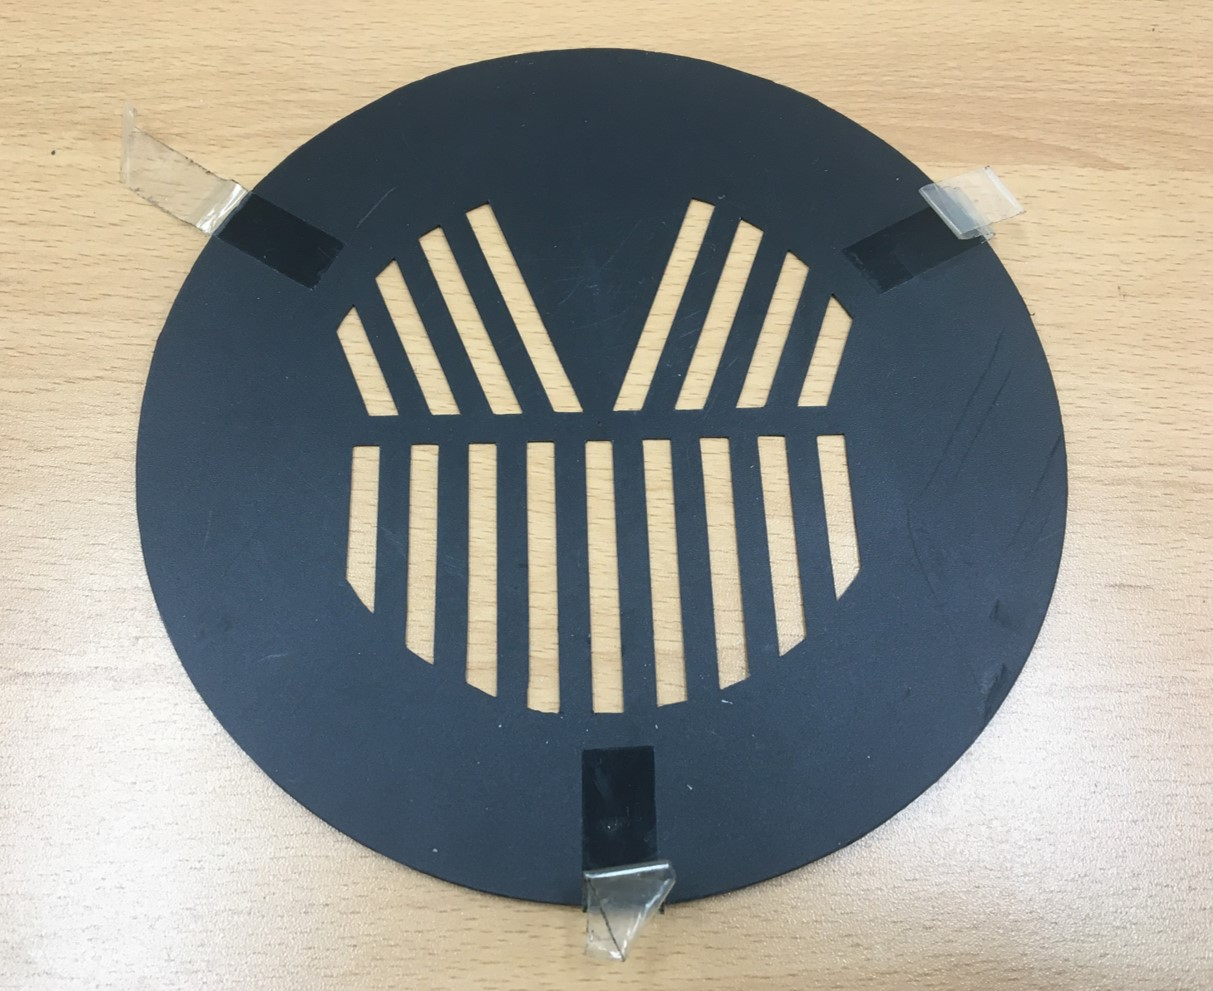
\includegraphics[width = 8cm]{bahtinov1}
	\end{center}
	\caption{실제로 천체관측에서 사용되는 바흐티노프 마스크}
	\label{bahtinov}
\end{figure}

바흐티노프 마스크는 빛의 회절을 이용하여 초점이 정확한지 여부를  쉽고 빠르게 알 수 있기 때문에 관측시간이 중요한 천체망원경의 초점을 맞추는 데 안성맞춤이다. 회절 슬릿을 이용하기 때문에 아주 밝은 별로만 초점 검출을 할 수 있다는 단점을 가지고 있지만 상대적으로 노출의 시간을 늘리는 밤에 천체관측을 할 때는 바흐티노프마스크가 좋은 선택이라고 할 수 있다.
(보완해야합니다)


\subsection{기존 모터포터서 분석 (기존에 존재하는 모터포커서 시스템)}


이전에 개발된 모터포커서인 GS-touch는 초점을 맞추기 위한 포커서이기 때문에 이를 위한 기능들이 주를 이루었다. 때문에 이를 보완하여 덮개를 제어할 수 있도록 추가로 개발할 필요가 있다.


Fig. \ref{GStocuh}는 기존에 사용하는 GS-touch의 주요 기능들을 정리한 표이며, GS-touch는 전체적으로 두 가지 부분으로 나눌 수 있다.
\bigskip
\begin{figure}[h]
	\begin{center}
		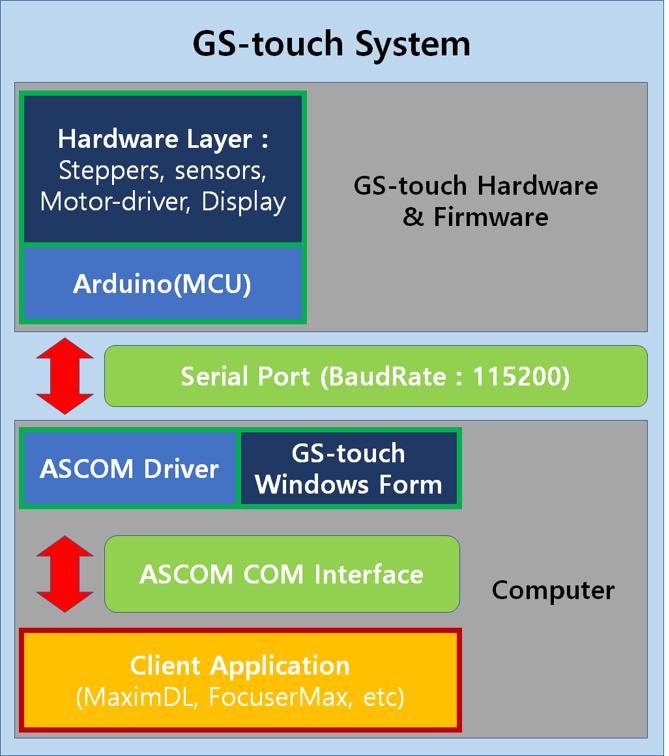
\includegraphics[width = 9.7cm]{GStouch}
	\end{center}
	\caption{GS-touch의 주요 기능}
	\label{GStocuh}
\end{figure}

첫 번째로 GS-touch의 펌웨어는 모터를 직접적으로 제어할 수 있다. DRV8825 모터 드라이버를 활용하여 최대 1/32step의 마이크로 컨트롤을 지원하기 때문에 정밀하게 경통의 길이를 조절할 수 있도록 설계되었으며, 이들을 편하게 관리할 수 있도록 움직인 만큼의 step을 디스플레이에 나타내주며, 이를 원하는 숫자로 초기화하여 얼마나 더 움직였는지 또한 알기 쉽게 하였다. 부가적인 기능으로는 현재 컨트롤러의 위치의 온도와 습도를 알 수 있도록 하여 주변 상황을 쉽게 알 수 있도록 하였다.

두 번째 부분은 GS-touch의 직접적인 제어가 가능하도록 하는 ASCOM 호환 드라이버이다. GS-touch의 드라이버는 ASCOM 홈페이지에서 제공하는 개발자용 버전을 응용하여 C\# 기반으로 제작되었으며, GUI 및 애플리케이션 소프트웨어를 제공하기 때문에 펌웨어에서 제공하는 모든 기능들을 컴퓨터에서 원격으로 사용할 수 있도록 하였다.


비록 GS-touch는 여러 가지 기능을 가지고 있지만 천체망원경의 원격조작에 필요한 여러 기능들을 완벽하게 갖추지는 못하였다. 대표적으로, EEPROM을 사용하지 않았기 때문에 원하는 길이에 step값을 저장할 수 없으며, 온도 및 습도 측정 외의 편의기능 또한 없기 때문에 실제로 사용할 때 많은 불편함이 있다. 본 연구에서는 이러한 단점들을 보완하여 EEPROM을 적용시키고 열선을 사용가능하도록 하는 등의 여러 편의기능들을 개선하였으며, 이를 사용하여 천체망원경용 덮개를 제어할 수 있도록 하였다. 앞으로 실제 천체관측에서의 활용성은 기존에 없었던 천체망원경용 덮개와 더불어 천체망원경의 원격 조작에 큰 도움을 줄 수 있을 것이다.

\subsection{천체망원경용 덮개}

천체 관측시에 덮개는 실제 관측상황시에도 여러 도움이 되지만, 관측을 하지 않는 상황에서 덮개는 큰 역할을 한다. 천체 망원경의 특성상, 보관할 때에 발생할 수 있는 여러 외부에서의 영향을 최소화하기 위해 덮개를 사용하는 것이 대부분이다. 덮개는 이슬 및 비의 영향에서 망원경을 보호할 수 있으며, 렌즈에 미치는 먼지와 같은 여러 가지 변수로부터 천체망원경을 보호할 수 있다. 때문에 천체망원경을 최적의 상태로 보관하기 위해서는 덮개를 사용하는 것이 효율적이다. 

때문에 초기 단계에서는 바흐티노프 마스크와 순수한 덮개의 용도의 두 단계의 덮개를 계획하였으나, 본 연구에서 사용된 천체망원경인 FSQ-106ED의 경우 본교의 돔스크린이 있는 천체관측소에 보관되고 있기 때문에 먼지와 같은 외부요인에 의한 영향이 거의 없기 때문에 최종적으로는 천체관측의 자동화에 도움을 줄 수 있는 바흐티노프 마스크의 제어용으로 덮개를 제작하였다.


\newpage
\section{연구 과정 및 방법}
\subsection{후드 제작}
본 연구에서는 Fusion360을 이용하여 경통의 후드를 제작하였다. 경통의 후드는 천체망원경 별로 경통의 지름과 같은 특성이 다르고, 천체망원경 위에 고정시킬 수 있을 만큼 견고해야한다. 때문에 경통에 씌울 수 있도록 지름을 계산하여 팔각형 모양으로 감싸는 형태로 제작하였으며, 3D프린터를 이용하여 제작을 편리하게 함과 동시에 천체망원경에 부착시킬 때 편리하게 할 수 있도록 총 네 조각으로 나누어 조립하는 방식을 택하였다.

\bigskip
\bigskip
\begin{figure}[h]
	\begin{center}
		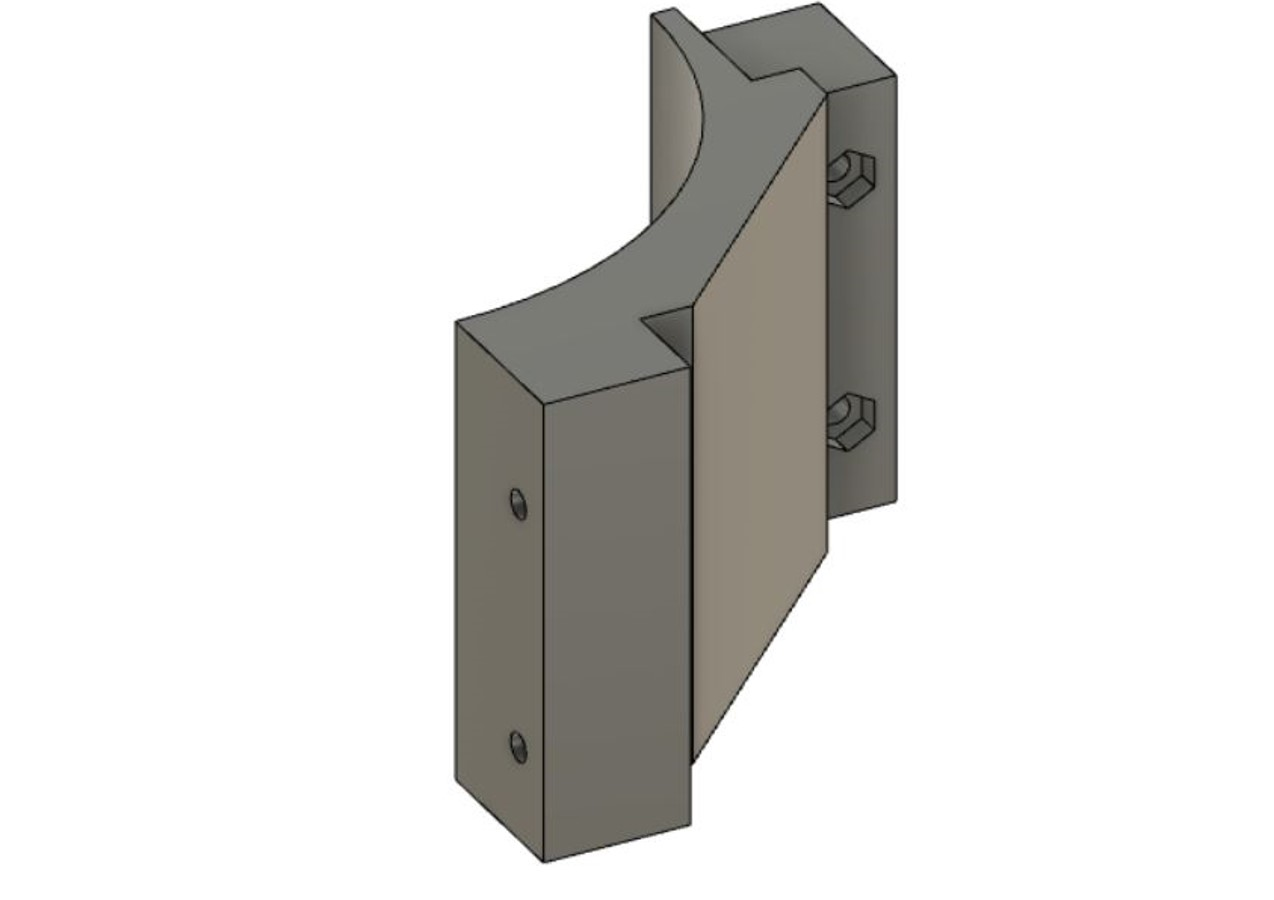
\includegraphics[width = 5.5cm]{coverpeice1}
		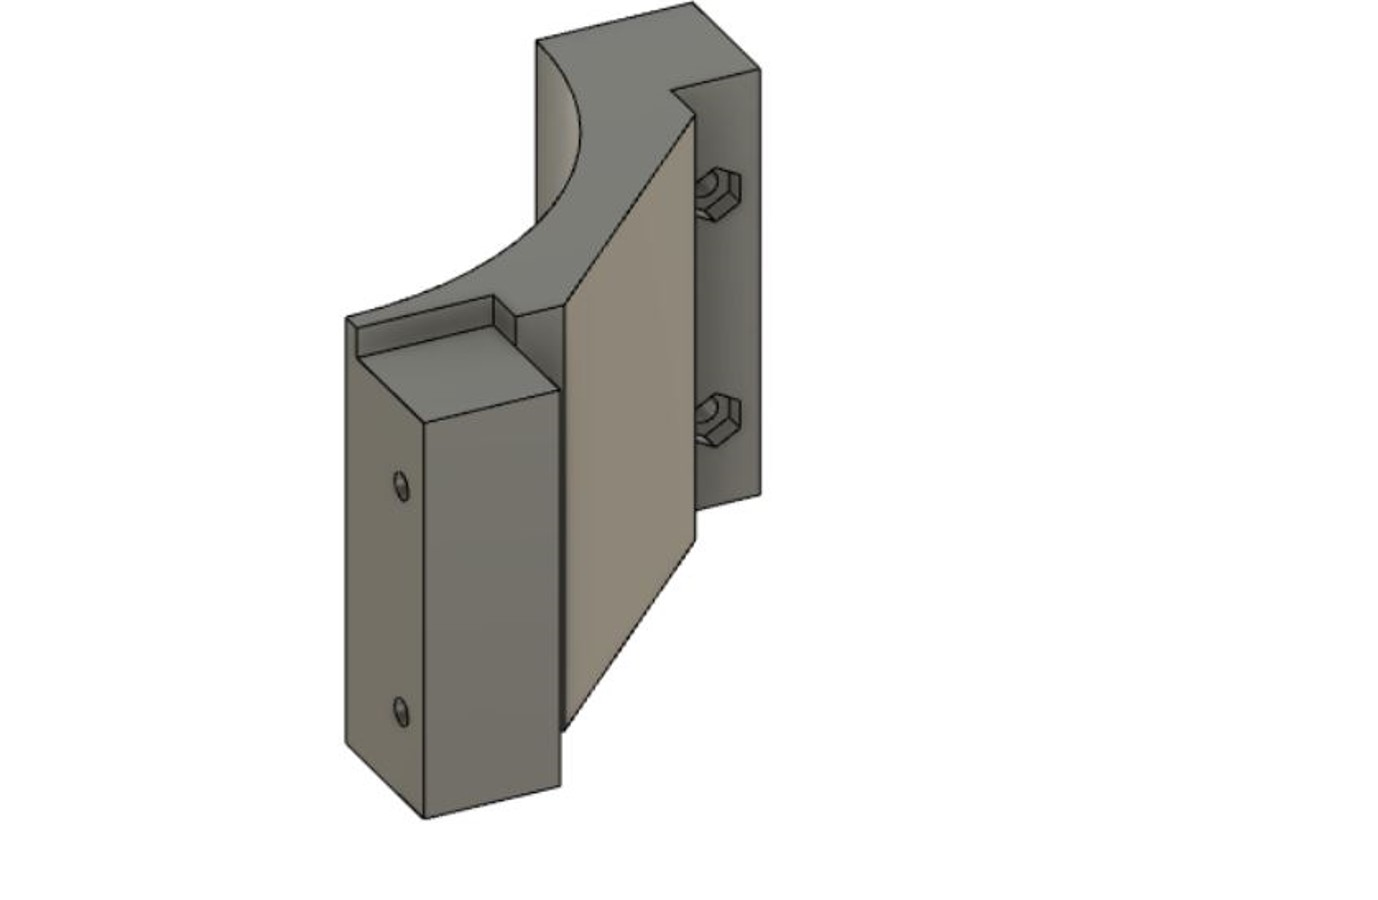
\includegraphics[width = 6cm]{coverpeice2}
	\end{center}
	\caption{Fusion360을 이용하여 설계한 경통 덮개조각들}
	\label{coverpeice}
\end{figure}

경통의 후드에서 바흐티노프마스크를 확실하게 제어하기 위해서는 바흐티노프마스크를 적용할 때와 적용하지 않을 때의 구분이 확실해야한다. 이를 확실하게 하기 위해서 바흐티노프마스크를 경첩을 이용하여 큰 각도로 제어하는 방법을 택하였으며, 이를 위해 덮개를 설계할 때 Fig. \ref{coverpeice}와 같이 경첩의 높이를 고려하여 제작하였다.

\subsection{바흐티노프마스크 제작}
천체망원경에 사용되는 대부분의 바흐티노프마스크의 도안은 직접 제작이 가능하며, 본 연구의 경우 astrojargon (http://astrojargon.net/MaskGenerator.aspx?AspxAutoDetectCookieSupport=1) 사이트에서 망원경의 사양 및 마스크의 사용 목적에 맞는 적절한 바흐티노프마스크의 도안을 제작하여 사용하였다.

덮개에서 사용되는 방식을 이용한 바흐티노프마스크의 경우 기존처럼 종이나 알루미늄에 프린트된 방식일 경우 덮개에 원하는 모양으로 씌워지지 않을 가능성이 있다. 때문에 주변환경에 영향을 적게 받으면서도 그 면이 평평하여 천체관측을 진행할 때에 영향이 없어야 한다. 


연구 초기에는 아크릴이 이러한 성질을 만족하면서도 쉽게 제작할 수 있으므로 아크릴에 레이저를 쐬여 바흐티노프마스크 모양을 씌우는 방법으로 테스트용 마스크를 제작해보았으나. 이러한 방식을 사용할 경우 Fig. \ref{bendmask}처럼 레이저로 인해 열을 받은 아크릴이 휘어 정밀한 초점 조절이 불가능해지는 경우가 발생하였으며, 아크릴의 두께로 인해 실제로 초점을 조절할 때에 걸리는 여러 가지 변수또한 무시할 수 없었다.

\bigskip
\begin{figure}[h]
	\begin{center}
		
\includegraphics[width = 12 cm]{bendmask}
	\end{center}
	\caption{레이저에 의해 휘어진 아크릴 마스크}
	\label{bendmask}
\end{figure}


때문에 선택한 새로운 방법은 3d프린터를 이용하여 바흐티노프 마스크를 출력하는 것이다. 이러한 방법을 사용하면 얇으면서도 딱딱한 마스크를 사용할 수 있으므로 일반적인 아크릴을 활용한 마스크보다 적은 변수로 바흐티노프 마스크를 덮개에 부착시킬 수 있다.
\subsection{서보모터 제어}
바흐티노프마스크를 제어하기 위해서 필요한 조건을 여러 가지가 있겠지만, 가장 중요한 조건 중 하나는 마스크를 사용하는 때와 그렇지 않을 때를 정확히 구분해야하며, 특히 마스크를 사용할 때에는 모든 상황에서 같은 환경을 제공할 수 있어야 한다. 본 연구에서는 경첩을 이용한 각도의 차이로 마스크를 제어하기 때문에 정확한 각도의 이동이 가장 중요하기 때문에 원하는 각도로 정확히 이동할 수 있는 서보모터를 사용하여 정확한 제어가 가능하도록 하였다.


서보모터는 일반적으로 사용하는 DC모터와 다르게 원하는 각도로 모터의 속도를 조절하여 이동시킬 수 있는 모터로,  RC카의 방향제어, 로봇의 관절제어 등의 상황에서 자주 사용되곤 한다. 본 연구에서 사용되는 서보모터는 ‘ds lx3325mg 25kg’ 모델(Fig. \ref{motor})으로, 서보모터이지만 360도 회전이 가능한 모델으로, 몸체가 금속으로 되어있어 내구성을 기대할 수 있으며, 축이 톱니모양으로 되어 있기 때문에 제어가 편리하다는 장점을 가지고 있다.

\begin{figure}[h]
	\begin{center}
		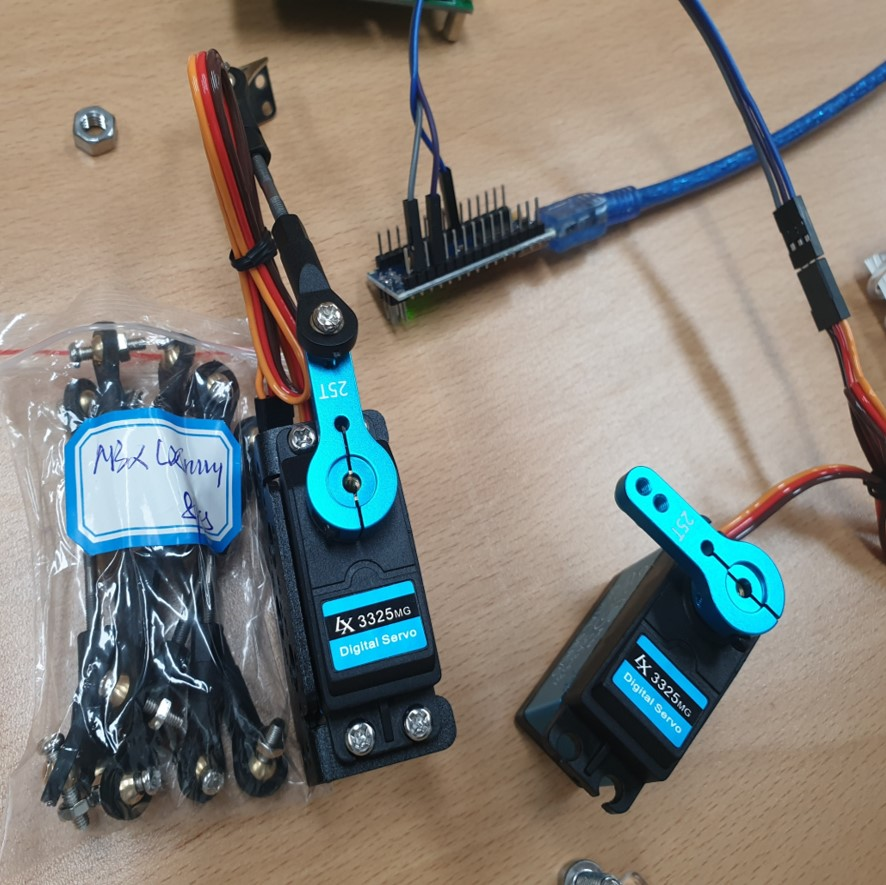
\includegraphics[width = 7cm]{servo1}
	\end{center}
	\caption{사용한 서보모터인 ds lx3325mg 25kg}
	\label{motor}
\end{figure}

\subsection{기존 모터포커서 보강}

앞서 소개했듯이 기존의 모터포커서인 GS-touch는 모터의 초점을 맞추기 위한 기능들에 집중이 되어있기 때문에, 실제로 천체관측 및 원격 천체관측에서는 사용하기 아쉬운 부분들이 많았다. 이에 기존 모터포커서를 보강하였으며, 기존 모터포커서에 비해서 원격 천체관측에 필요한 여러 가지 기능들을 탑재하였다. 본 연구에서 새로 보강한 부분은 다음과 같다.
\subsubsection{열선 제어}
열선또한 정확한 천체관측에 필요한 장비 중 하나이다. 관측을 진행할 때에 경통의 온도가 내려가면 렌즈에 이슬이 맺히게 되는데, 이는 정확한 상을 맺히게 하는데 크게 어려움을 주게 된다. 열선을 경통에 감아놓으면 경통의 온도에 따라서 열선을 제어하여 깨끗한 렌즈를 사용할 수 있게되므로 관측을 편리하게 할 수 있으며, 때문에 천체망원경을 원격제어하기 위해서는 온도를 측정할 수 있는 장비와 열선이 필수적이다. 열선은 히팅게이블을 이용하여 제작하였으며, 망원경의 크기와 열의 필요세기 등을 고려하여 히킹케이블의 저항을 선택한다.

\begin{figure}[h]
	\begin{center}
		\begin{tikzpicture}
		\node[anchor=south west,inner sep=0] at (0,0) 
		{
			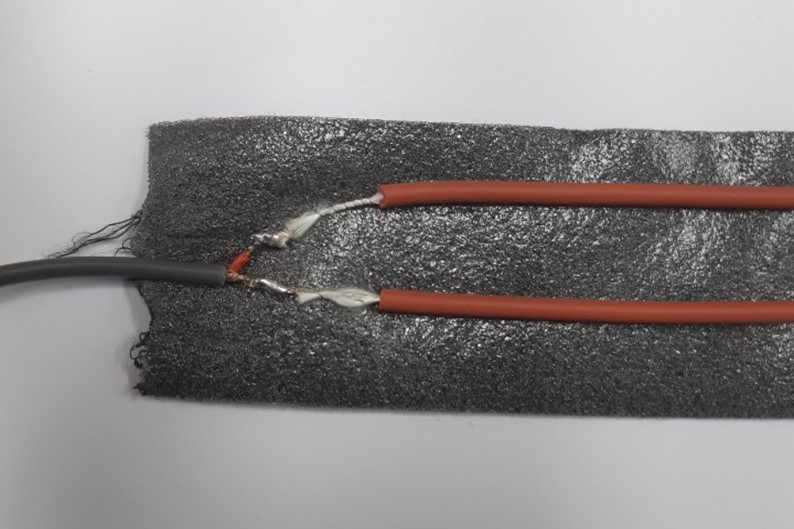
\includegraphics[width=6cm]{thermicline1}
			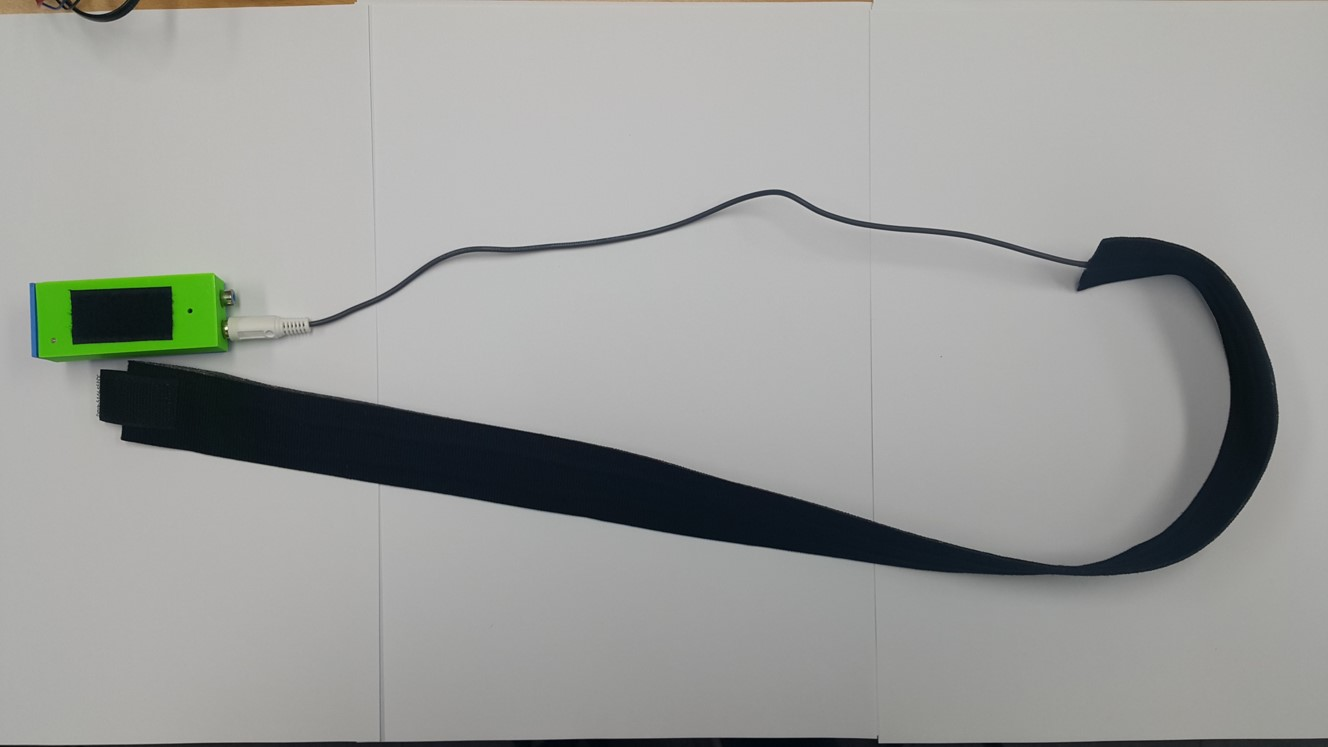
\includegraphics[width=7cm]{thermicline3} 
		};
		\draw (0.3, 3.7) node {(a)};
		\draw (6.4, 3.7) node {(b)};
		\end{tikzpicture}
	\end{center}
	\caption{(a) 제작한 열선의 접합부와 (b) 제작한 열선을 12V에 연결한 모습. 끝에 벨크로가 붙어있어 경통에 둘러 사용할 때 편리하다.}
	\label{thermic}
\end{figure}


열선을 제작하는 방법은 간단하다. 먼저 Fig. \ref{thermic}a처럼 끈끈한 면에 히팅케이블을 부착한 뒤에 알맞는 12V어댑터를 분해하여 극을 선과 연결한다. 그리고 열선을 다시 덮어주게 되면 12V 전원을 통해 작동하는 열선을 제작할 수 있다. 열선을 실제로 사용할 시에는 그 편의성을 증대시키기 위해 열선의 끝부분을 벨크로로 연결할 수 있도록 만들게 되며, 이렇게 제작한 열선은 렌즈가 있는 부분을 찾아 둘러주면 벨크로로 끝을 고정시켜 쉽게 망원경에 부착시킬 수 있다.

열선은 PWM(Puls Width Modulation)을 이용하여 세기를 조절할 수 있다. PWM은 디지털 신호의 밀도로 그 세기를 조절하는 방식으로다 디지털 신호인 0과 1이 출력되는 시간의 비율을 조절하여 원하는 밀도로 제어할 수 있도록 한다. 본 연구에서 직접 제작한 열선을 포함한 대부분의 열선은 12V의 전압을 이용해 제어해야하기 때문에 아두이노의 출력 전원인 5V로는 신호만 제어하고 스위칭 트랜지스터를 이용하여 12V의 전압을 PWM으로 제어할 수 있도록 설계하였다.

\subsubsection{EEPROM(Electrically Erasable Read-Only Memory)}

MCU(Micro Controller Unit)내에 원하는 값을 저장하는 방법은 여러 가지가 있다. 일반적으로 펌웨어가 실행되기 전에 변수를 선언하고, loop 문 속에 들어있는 여러 함수들을 통해 그 값을 바꾸는 방법을 사용하곤 한다. 하지만 원격 천체관측을 위한 펌웨어인 만큼, MCU내의 변수만으로 값을 저장하는 것은 상당히 위험하며, 그 전원을 계속 유지할 수 없기 때문에 다른 방법으로 값을 저장할 필요성을 느꼈으며, EEPROM은 기존 방법에 비해 안전하게 값을 저장할 수 있기 때문에 사용하게 되었다.

EEPROM은 대표적인 롬(ROM - read only memory)의 한 종류로서, 전원을 차단해도 저장된 정보를 유지하는 비휘발성 메모리이다. EEPROM은 address를 가지고 있어서 각각의 address 안에 지정된 bytes의 값을 저장할 수 있다. 본 연구에서 사용된 MCU인 Teensy 3.2는 0에서 1023까지의 address지를 가지고 있고 하나의 address에 2048byte, 즉 0부터 255까지의 수를 저장할 수 있다. 모터포커서의 step을 저장하기 위해서는 약 100000범위의 수를 저장할 필요가 있다. GS-touch는 약 -50000에서 50000까지의 수를 저장할 수 있기 때문에 256진법을 활용하여 수를 저장할 수 있도록 설계하였다.
\begin{figure}[h]
	\begin{center}
		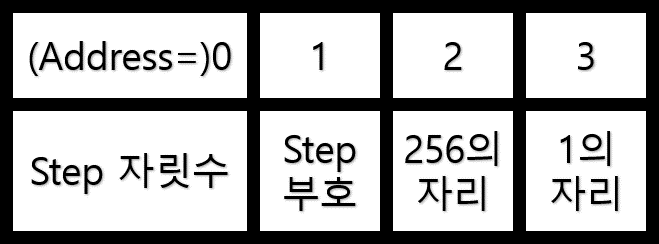
\includegraphics[width = 5 cm]{eeprom1}
	\end{center}
	\caption{EEPROM의 address별 사용 구조. 부호와 값을 절대치를 이용하여 연산하였다.}
	\label{eeprom1}
\end{figure}


%https://www.pjrc.com/teensy/td_libs_EEPROM.html


\subsubsection{서보모터 제어}

\begin{comment}
\begin{figure}[h]
\begin{center}
\begin{tikzpicture}
\node[anchor=south west,inner sep=0] at (0,0) 
{
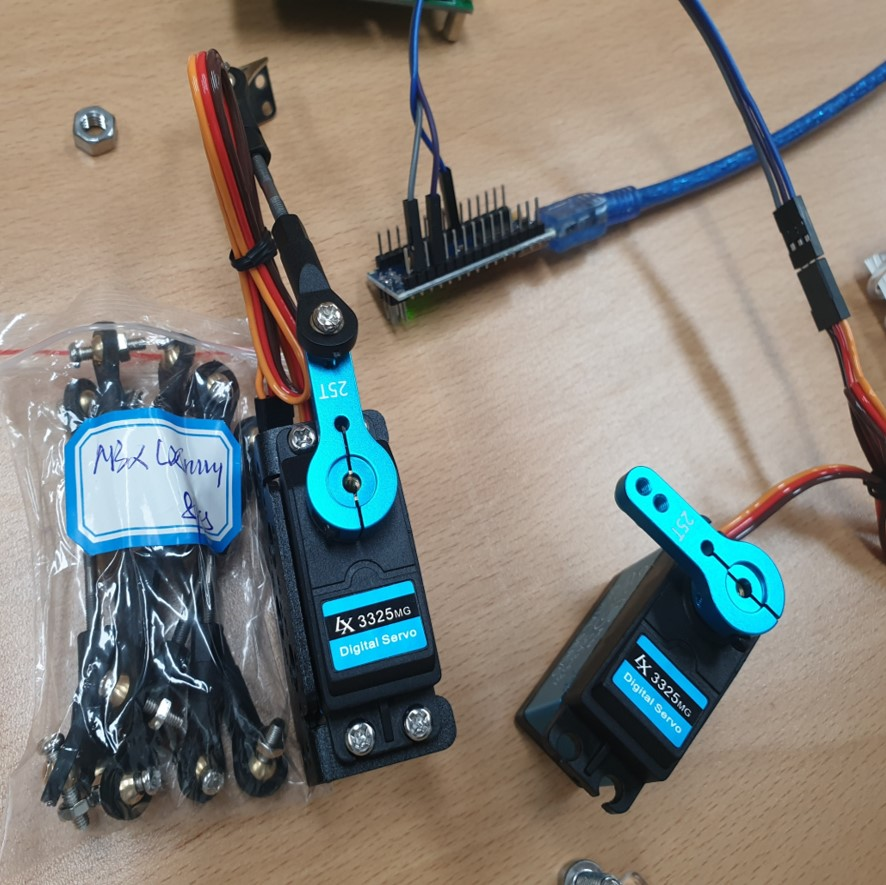
\includegraphics[width=6cm]{servo1}
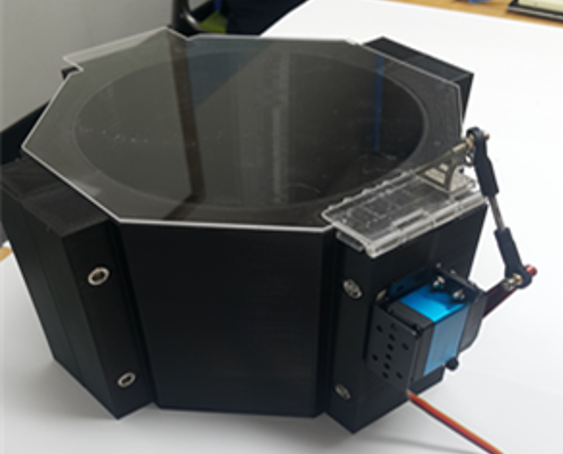
\includegraphics[width=6cm]{servo2} 
};
\draw (0.3, 5.7) node {(a)};
\draw (6.4, 5.7) node {(b)};
\end{tikzpicture}
\end{center}
\caption{(a) 사용한 서보모터인 ds lx3325mg 25kg와 (b) 이를 제작한 덮개에 장착한 모습.}
\label{motor2}
\end{figure}
\end{comment}

\begin{figure}[h]
	\begin{center}
		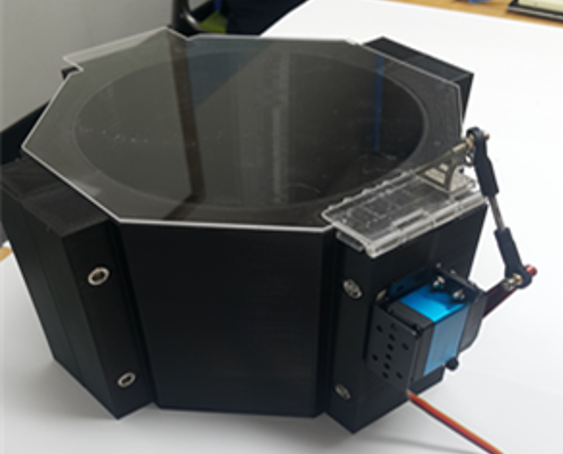
\includegraphics[width = 7.5cm]{servo2}
	\end{center}
	\caption{서보모터를 제작한 후드에 장착한 모습.}
	\label{motorcover}
\end{figure}

서보모터의 경우 구동을 위해 필요한 핀은 3가지이며, 일반적으로 주황색, 빨간색, 갈색의 핀으로 이루어져 있다. 주황색 핀은 모터를 제어할 수 있는 핀이며, 빨간색 핀과 갈색 핀은 각각 5v 전원과 GND에 연결하여 서보모터를 구동할 수 있다. 서보모터의 경우 Fig. \ref{motorcover}처럼 후드의 옆면에 부착시켜 일정한 각도로 제어할 수 있게끔 설계하였다.


\subsubsection{릴레이 스위치}

\begin{figure}[h]
	\begin{center}
		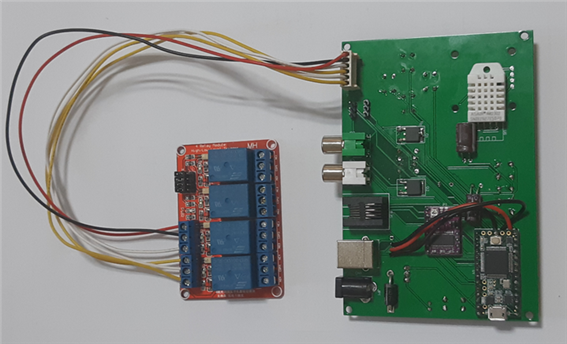
\includegraphics[width = 7.5cm]{relay}
	\end{center}
	\caption{실험에 사용된 릴레이스위치를 모터포커서에 연결시킨 모습}
	\label{relay}
\end{figure}



릴레이 스위치는 전자석으로 이루어진 여러 스위치를 한번에 제어할 수 있도록 제작된 장비이다. 천체관측을 시작 및 종료할 때 가대, CCD, 카메라 등 한번에 여러 가지의 전원을 제어해야 하는데, 릴레이 스위치를 이용하면 한번에 제어할 수 있어 편리하다. 


Fig. \ref{relay}와 같이 각각의 스위치를 선으로 연결시켜 mcu의 각 핀에 연결시켜 작동시킬 수 있으며, 함수로 지정하여 이들을 한번에 제어할 수 있도록 하였다.